\begin{figure*}
\centering
%\mbox{
  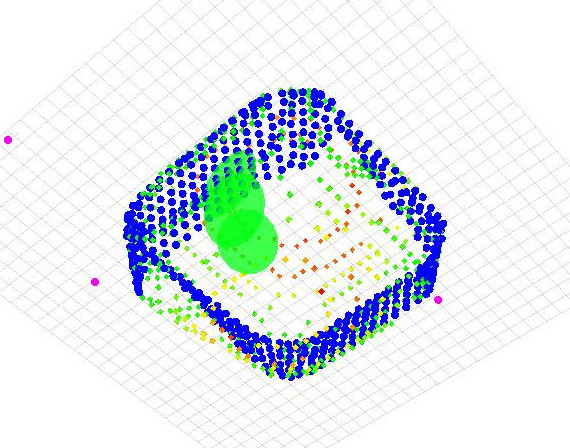
\includegraphics[width=0.45\textwidth]{next_best_touch.jpg}
  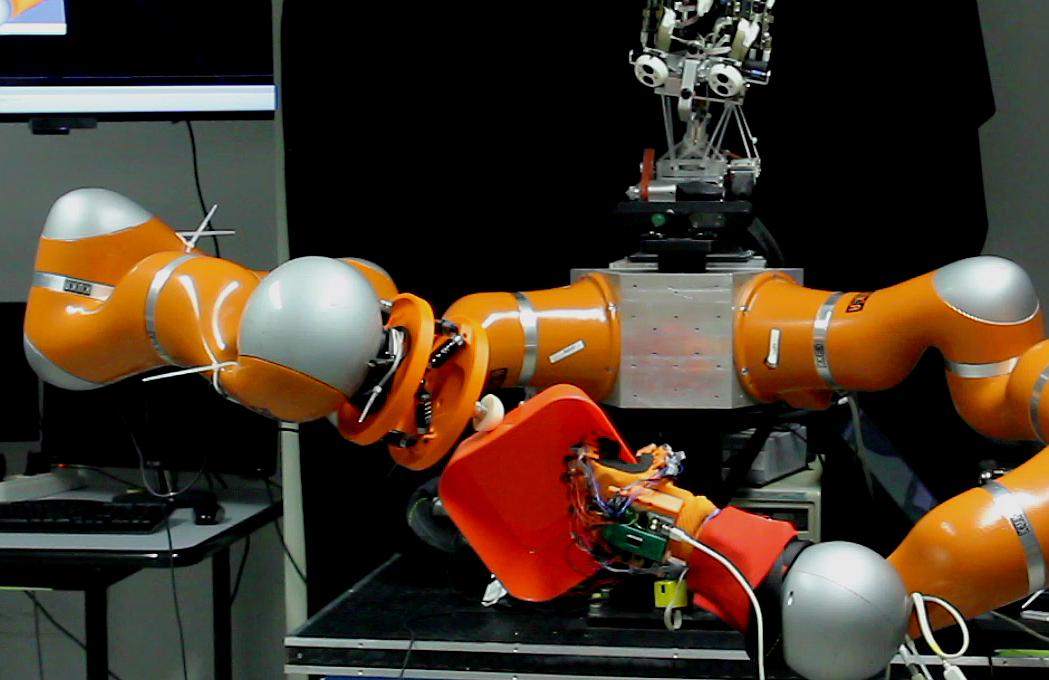
\includegraphics[width=0.53\textwidth]{intro_vito.png}
%}
\caption{(Left) The GPAtlasRRT strategy suggests touches (light green coloured disks) on the predicted surface. The blue points show the initial partial reconstruction from a depth camera that the robot uses to guide tactile search. The predicted surface is also shown as points coloured from green to red. Green indicates high uncertainty in the surface prediction, and red indicates low uncertainty. (Right) Our Vito robot executing a step of tactile exploration.}
\label{fig:setup_solution}
\end{figure*}

% why the problem we are dealing with is important
Recovery of the properties of a new object is a basic task in robot manipulation. Properties of interest include object shape, texture, friction coefficients, elasticity, plasticity, etcetera. Because the object is initially unknown the sensing strategy must be active, i.e.\ the robot must adapt its sensing actions based on the results so far. A popular modality for active sensing is vision. Active vision has been studied in depth for the problem of shape and pose recovery for robot grasping\cite{Kragic2002TechRep,nunez2013models,arruda16,kopicki2015ijrr,kootstra2012a}. Humans, however, also use active tactile sensing \cite{johansson92}. There is a variety of work on tactile exploration for robot manipulation \cite{zito2013sequential,jentoft2014a,Bjorkman2013Enhancing,Hebert2013Next,Petrovskaya2011Global}. The goal of this paper is to extend the set of available techniques for guiding tactile exploration to recover surface shape.

The requirements for active tactile perception were authoritatively spelled out by Bajcsy and co-workers\cite{Bajcsy1988Active} in the 1980's. Early tactile perception algorithms date back to the same period \cite{Grimson1984JRR,Faugeras1983IJCAI,Shekhar1986ICRA,Bajcsy1989Machine}. Active touch, however, lags behind active vision for two reasons. The first reason concerns robot hardware. Standardized touch sensors are still not widely available and typically have to be hand crafted or modified for the specific robot and task. The second reason is intrinsic to touch itself, which requires the mechanical interaction of the sensor and the object being perceived. This inevitably leads to unexpected perturbations of the sensor and object, which in turn require rather complex control of the ongoing movement of the sensor: a requirement which is absent in vision.

In this paper, we suppose that vision has already provided some partial information about the shape of the object. Given this initial, partial, surface model our method plans a  sequence of touches. The planning relies on the ability of the robot to form hypotheses about the shape of the hidden parts of the object. The robot then attempts to touch the surface, so as to refine these hypotheses. Whether or not a contact is made the information gained improves the model of the object shape.

Tactile information is sparse, and so refining beliefs about the shape must use data-efficient inference. We follow others working on tactile estimation of surface shape \cite{Dragiev2011Gaussian,Bjorkman2013Enhancing,Sommer2014Bimanual} by employing Gaussian Process (GP) inference \cite{Rasmussen2006Gaussian}.  This produces data-efficient, nonlinear regression estimates of the object's surface shape. It also predicts the variance in these surface estimates. The surface is implicitly defined, being the $0$-levelset of an \emph{unknown} function. This implicit surface representation is also well established.

Given this combination of a representation and an inference method the remaining issue is how to explore the object surface so as to generate the data points. The criterion that we use to drive exploration is reduction of uncertainty in object shape, again similar to that deployed in previous work. Where we diverge is in the planning to achieve this reduction. In order to plan sequences of touches, rather than merely a solitary touch, it is handy to interpret the implicit surface as a manifold. We can then build a tactile exploration planner using recent methods for sample-based exploration of general manifolds~\cite{Jaillet2013Path}. 

In more detail, given an implicitly defined surface prediction, we build a collection of charts (an atlas) that model the shape, and use these to perform a search across the object, driven towards areas of high uncertainty in the implicit surface. The construction of the atlas follows as well as drives the exploration. Specifically, we search for points on the estimated surface that have a variance larger than some pre-specified threshold. The expansion and planning process is repeated after execution of each touch. By repeated touches the robot will converge on an estimated surface, such that any point on it has low variance. The terminating condition is met when no candidate for the next best touch is found by the GPAtlasRRT algorithm, which means the that object shape prediction meets the requirement on variability. Naturally, the smaller the threshold (i.e. the more accurate the model is required to be), the higher the number of touches required to converge. This threshold is the only input to the devised strategy, given either by a higher level module or the user.

The structure of the paper is as follows. In Sec.~\ref{sec:related} we first review previous work related to tactile exploration and object shape representation. In Sec.~\ref{sec:scope} we clearly state the problem we aim to solve and in Sec.~\ref{sec:solution} we present the envisioned approach for its solution. The experimental results and their discussion are presented in Sec.~\ref{sec:experiments}. Finally, conclusions and points deserving further attention are given in Sec.~\ref{sec:conclusions}.

% why tactile exploration is not so developed
% and what makes the problem harder that active vision

% why we propose touch (Bajcsy) and why ITS

% what is exactly our contribution

% RELATED WORK

% only localization

% also shape reconstruction
% they also use GP

% what are we doing more at least in surface exploration?
% we are exploiting the implicit manifold nature of GP representation
% and adapt efficient sample-based method for exploring the manifold in
% an intrinsic  way.



%General guidelines : \cite{Bajcsy1989Machine}
%
%Active visual perception: \cite{Bajcsy1988Active}
%
%Vision-based exploration is the most studied, perhaps due to its non-invasive nature, which avoids the contact between rigid bodies which is the cause of most headaches in physics modelling, simulation and control.
%
%As very well said by \cite{Petrovskaya2011Global}, even when initial works date back to the 80's, tactile perception has not been addressed as deeply as the non-invasive counterpart, visual perception. Besides the need of being actively controlled, tactile sensors typically required ad-hoc mechanical devices.
%
%``Touch-based perception has not been studied in as much depth
%as vision because standardized touch sensors are not as easily
%available. In many situations, tactile sensors have to be hand
%crafted specifically for the robot and the task. This complicates
%comparisons between methods and slows progress in tactile
%perception. However, recently there has been a surge of interest
%in the field due to the necessity of touch-based perception in
%service applications''
%
%Whereas \cite{Petrovskaya2011Global} is more interested in the object pose estimation problem, here we are more interested in the object shape modelling, sort of in the mapping of rather than localization in a SLAM problem.
%
%On active touch sensing \cite{Prescott2011Active}
%
%Differentiate from active touch for localization, here another example: \cite{Hebert2013Next}.
%
%Justify the use of a intrinsic tactile sensor over a tactile array.
%
%ITS are more precise and less noisy. It provides the contact normal directly in sensor frame.
%
%Tactile arrays provide multiple-point measurements. They do not provide directly the normal in sensor frame, forward kinematics is required over noisy joint measurements, or in fixed configurations that limit exploration mobility. Up to a point that a typically a complex framework is needed to exploit its grasping and touching properties % cite http://www.roboticsproceedings.org/rss09/p45.pdf?
%
%With ITS, the computation will be trivial. The disadvantage is that it is a single-point measurement. Poking strategies, like in~\cite{Petrovskaya2011Global}, or trajectories strategies like in~\cite{Rosales2014Active}.
%
%% They claim that touch sensing is low bandwith, local, sequential process with better signal-to-noise ratio than vision.
%
%% Vision is global, has high bandwidth, and is noisy. Touch is a low bandwidth, local, sequential process with better noise properties than vision.
%
%%% Finish the introduction with some motivation
%On how to do classification...
%
%Shape representation and descriptor review \cite{Zhang2004Review}
%
%In this work, we provide a systematic methodology to plan the next-best tactile exploratory action. The tactile exploratory action is intrinsically a contact hypothesis that need to be accepted or discarded after execution. Should the result be any of the two, it helps to improve the object shape prediction up to a pre-specified variability. In contrast to \cite{Bjorkman2013Enhancing}, we propose the same shape representation as descriptor for classification purposes using shape matching techniques~\cite{Belongie2002Shape}. The scope and problem statement is detailed in Sect.~\ref{sec:scope}. The proposed solution is broaden in Sect.~\ref{sec:solution}. The experimental results and discusion is presented in Sect.~\ref{sec:experiments}. Finally, the conclusions and points deserving further attention as given in Sect.~\ref{sec:conclusions}.
%%Reading the paper along watching the attached media is suggested for a better cath-up of the ideas.
